% !TEX root = ./w26-L13-transformers.tex
\documentclass{article}
\usepackage[a4paper,margin=1in]{geometry}
\usepackage{calc}
\usepackage{amssymb}
\usepackage{polynom}
\usepackage{amsmath,amssymb,amsthm}
\usepackage{graphicx} 
\usepackage{xcolor}
\usepackage{float}

\definecolor{lightblue}{RGB}{100,149,237}
\newcommand{\dimlabel}[2]{\underset{\color{lightblue}{#2\strut}}{#1}}

\setlength{\parindent}{2em}
\setlength{\parskip}{0.55em}

\newcommand{\lectureheader}[4]{
	\setlength{\fboxrule}{0.4pt}
	\setlength{\fboxsep}{10pt}
	\noindent\fbox{%
		\begin{minipage}{\dimexpr\textwidth-2\fboxsep-2\fboxrule\relax}
			{\small\hfill #1\par}
			\vspace{0.6em}
			{\centering\LARGE\bfseries #2\par}
			\vspace{0.9em}
			{\small\itshape\noindent Lecturers: #3\hfill Notes: #4\par}
		\end{minipage}%
	}
	\vspace{1.2em}
}

\begin{document}

\lectureheader
	{COMP 551 -- McGill, Winter 2026}
	{Topic 13: Attention Mechanism \& Transformers}
	{Siamak Ravanbakhsh \& Pascale Gourdeau}
	{Raphaël Michnik}

\textbf{Certification:} I wrote these notes myself, without any LLMs

\section{Attention Mechanism}

\subsection{Motivation: Models for Sequence Data}

When processing sequence data, different architectural families use different inductive biases to capture patterns. Convolutional Neural Networks (CNNs) rely on translation invariance and locality, computing outputs as a weighted sum of neighboring input units. Recurrent Neural Networks (RNNs) update a hidden state sequentially through time to summarize past observations. However, this creates a bottleneck in standard encoder-decoder architectures, because the whole input sequence has to be squeezed into a single context vector. Transformers avoid this by replacing recurrence with attention. Instead of passing information step by step through time, each position can look directly at the parts of the input that matter most. This helps the model capture long-range relationships and makes parallel computation possible.

\subsection{Idea}

When answering certain queries we should focus on relevant parts of data. In an image, that might mean looking at the region containing the object mentioned in a caption. More generally, for sequences or sets of elements, attention lets the model select and combine the most useful information to produce and output.

\begin{figure}[htbp]
    \centering
    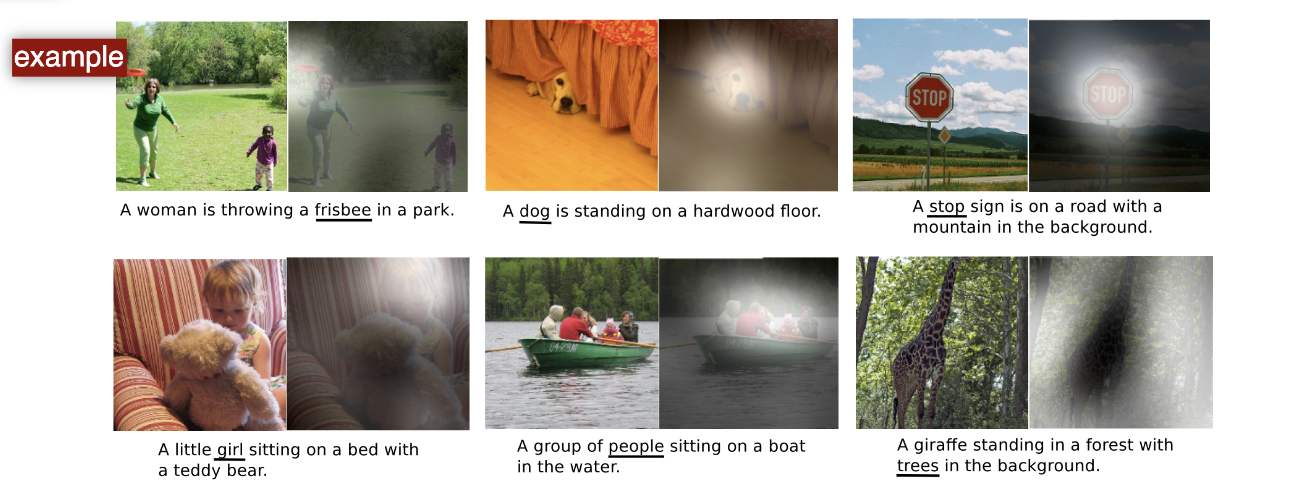
\includegraphics[width=0.8\linewidth]{images/attention_for_images_example.png}
    \caption{Example of attention in image captioning. When generating the word "dog", the model can focus on the region of the image containing the dog, rather than processing the entire image uniformly.}
    \label{fig:attention_for_images_example}
\end{figure}

\noindent Different parts of the input can have different importance depending on the query. The output can be generated by focusing on and combining the most relevant elements.

\subsection{Attention Mechanism}

\textbf{Objective:} Given a set of inputs vectors $x_1, \dots, x_T$ and a query vector $q$, create an output based on the query and the input. 

Each input vector $x_i$ is compared with the query to determine its relevance. These relecance scores are converted into weights, and the output is formed as a weighted combination of the input vectors.


For each input $x_t$ we construct a \textbf{key} $k_t$ and a \textbf{value} $v_t$. The key is used to determine how relevant that input is to the query, and the vlaue is the information that will contribute to the output. We might use $v_t = k_t = x_t$ or transformed versions $v_t = W_v x_t$ and $k_t = W_k x_t$.

First compare the query $q$ with each key $k_t$ using a scoring function, then apply a softmax functno so taht the scores become normalized attention weights $\alpha_t$ that sum to 1. Using softmax:

\[ \alpha_t(q, k_1, \dots, k_T) = \mathcal{S}(q^Tk_1, \dots, q^Tk_T) \]

\noindent The output is a weighted sum of values:

\[ \text{Attn}(q, (k_1, v_1), \dots, (k_T, v_T)) = \sum_{t=1}^T \alpha_t v_t \]

\begin{figure}[htbp]
    \centering
    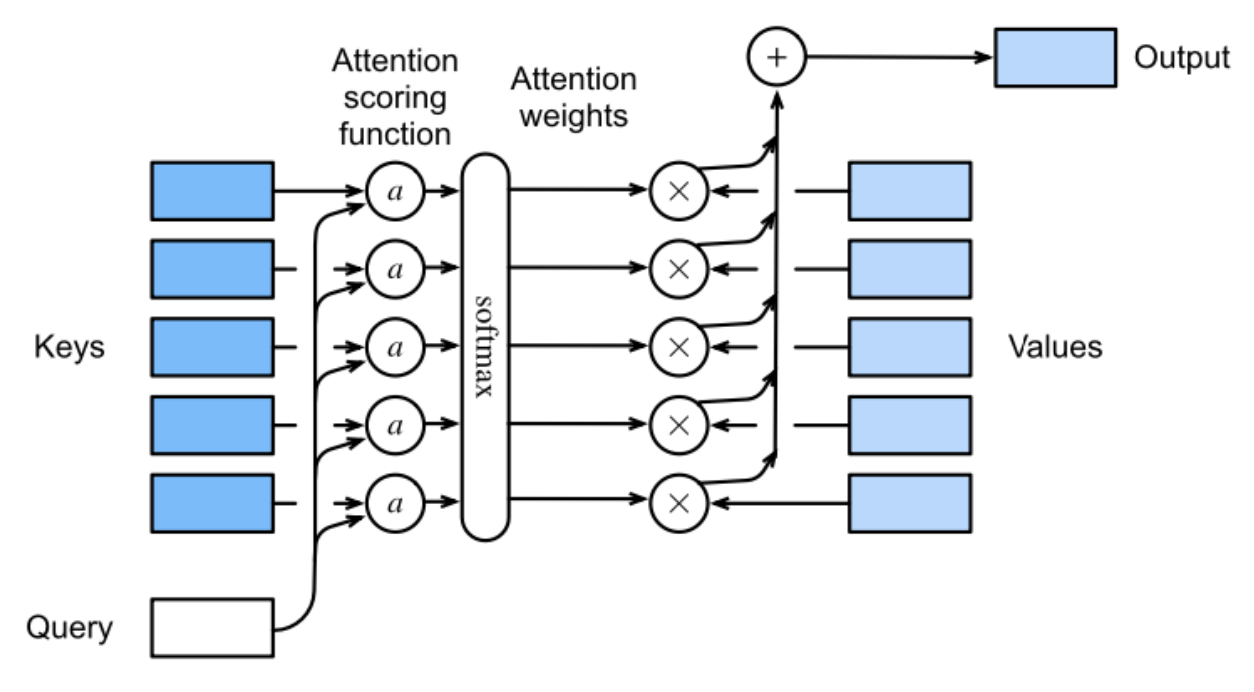
\includegraphics[width=0.6\linewidth]{images/attention_mechanism_diagram.png}
    \caption{Diagram of the attention mechanism. The query is compared with all keys to produce attention weights, which are then used to form a weighted sum of the value vectors.}
    \label{fig:attention_mechanism_diagram}
\end{figure}

\noindent There are many choices for the scoring function $a(q, k)$. The simplest is \textbf{dot-product attention:} $a(q, k) = q^T \cdot k$, assuming $q, k \in \mathbb{R}^D$. A common improvement is \textbf{scaled dot-product attention:} $\frac{q^T \cdot k}{\sqrt{D}}$, which doesn't scale with $D$. Another option is \textbf{additive attention:} $a(q, k) = w^T \cdot \tanh(W_q q + W_k k)$.

If all inputs are stacked into a matrix $X$, we can compute keys and values as 

\[
\dimlabel{K}{T \times D_k}
=
\dimlabel{X}{T \times D}
\dimlabel{W_k}{D \times D_k}
\quad\quad
\dimlabel{V}{T \times D_v}
=
\dimlabel{X}{T \times D}
\dimlabel{W_v}{D \times D_v}
\]

\[ \text{Attn}(q, K, V) = \mathcal{S}\dimlabel{(qK^T)V}{D_v}\]

\noindent \textbf{Example: SeqToSeq with Attention:} Recall that the the context vector in encoder-decoder RNN is a "bottleneck", as all information must pass through one vector and long-range dependencies are hard to preserve. In tasks like translation, different output words depend on different parts of the input.

When generating each output word, the model should focus on different input words. Without attention, it cannot do this explicitly.

\begin{figure}[H]
    \centering
    \begin{minipage}{0.48\textwidth}
        \centering
        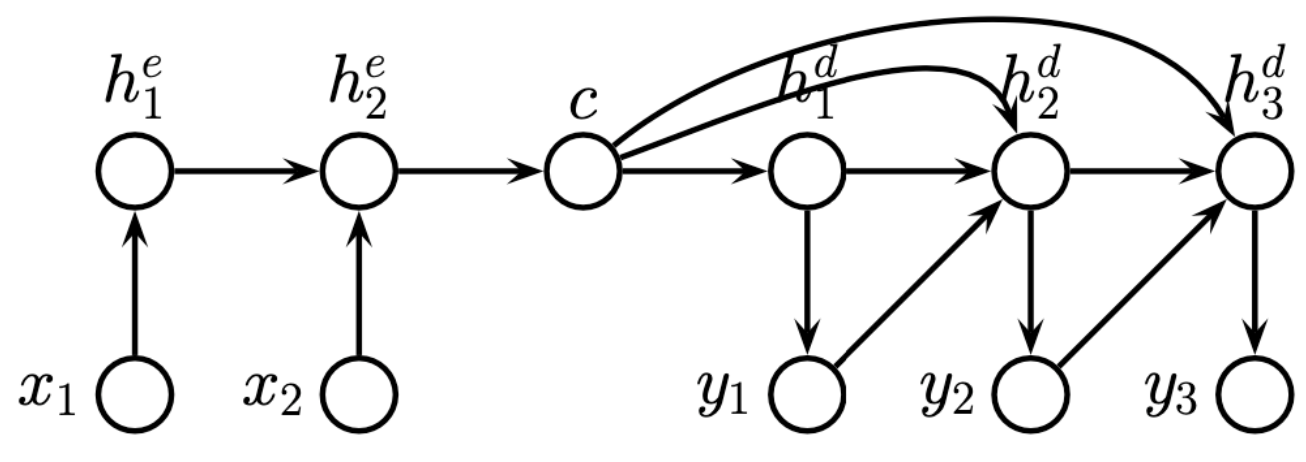
\includegraphics[width=\linewidth]{images/seq2seq-nn.png}
    \end{minipage}
    \hfill
    \begin{minipage}{0.40\textwidth}
        \centering
        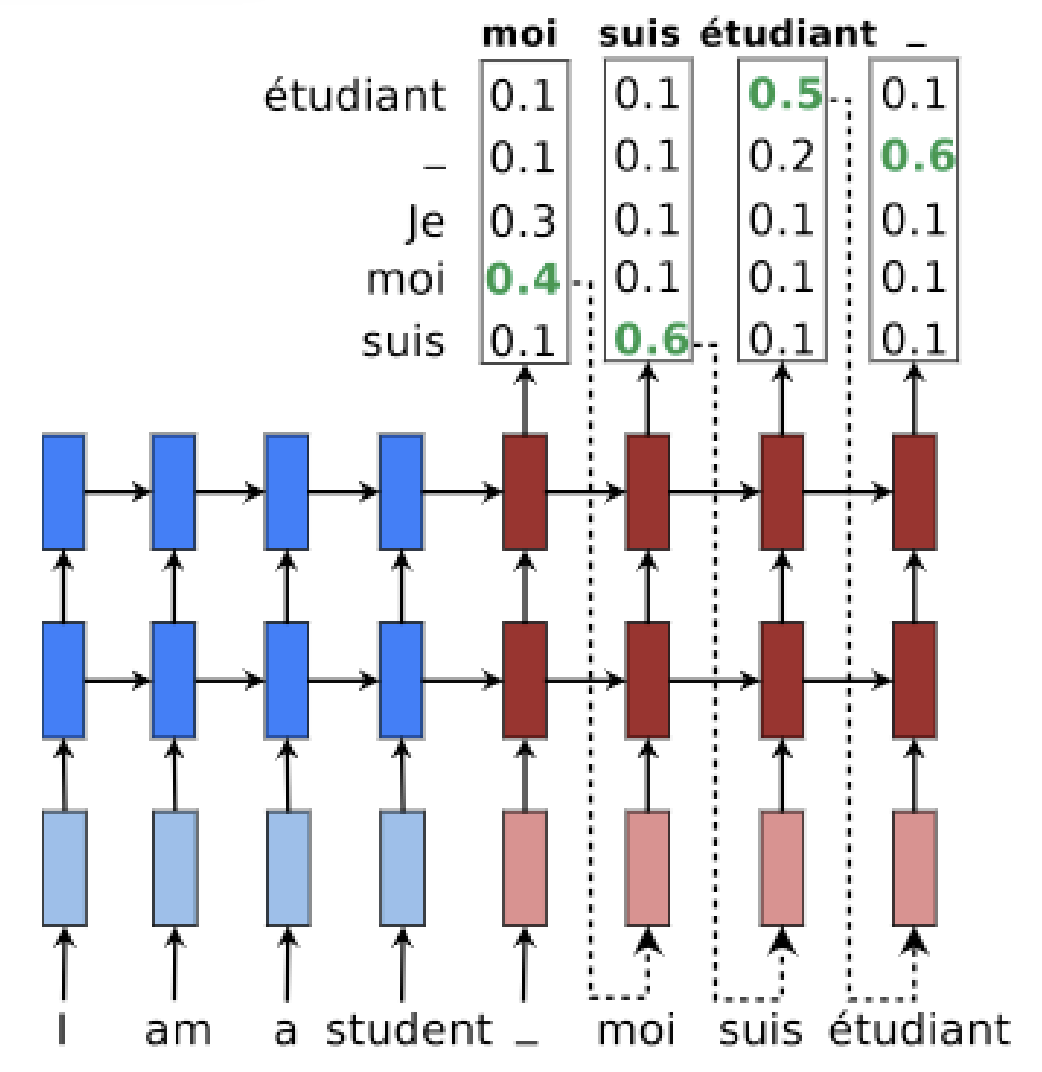
\includegraphics[width=\linewidth]{images/seq2seq-with-attention.png}
    \end{minipage}
    \caption{Neural Machine Translation without and with attention. The left diagram shows a standard encoder-decoder architecture where the encoder produces a single context vector that the decoder uses to generate the output sequence. The right diagram shows how attention allows the decoder to focus on different parts of the input sequence when generating each output word, improving performance}
    \label{fig:seq2seq-with-attention}
\end{figure}

\noindent Attention replaces the fixed context vector with a dynamic one that is recomputed at each decoding step. Instead of relying on a single summary, the decoder selectively focuses on different encoder states depending on what it is generating. This allows the model to align input and output elements and capture long-range dependencies more effectively.

At each decoding step, we compute a context vector:

\[ c_t = \sum_{i=1}^T \alpha_i (h_t^d, h_i^e)h_i^e \]

We compare the current decoder hidden state $h_t^d$ with each encoder hidden state $h_i^e$ to get attention weights $\alpha_i$. Then take a weighted sum of encoder states. The output depends on the decoder state and the context vector, the model is effectively "looking back" at the input each time it generates a word.

\begin{figure}[H]
    \centering
    \begin{minipage}{0.35\textwidth}
        \centering
        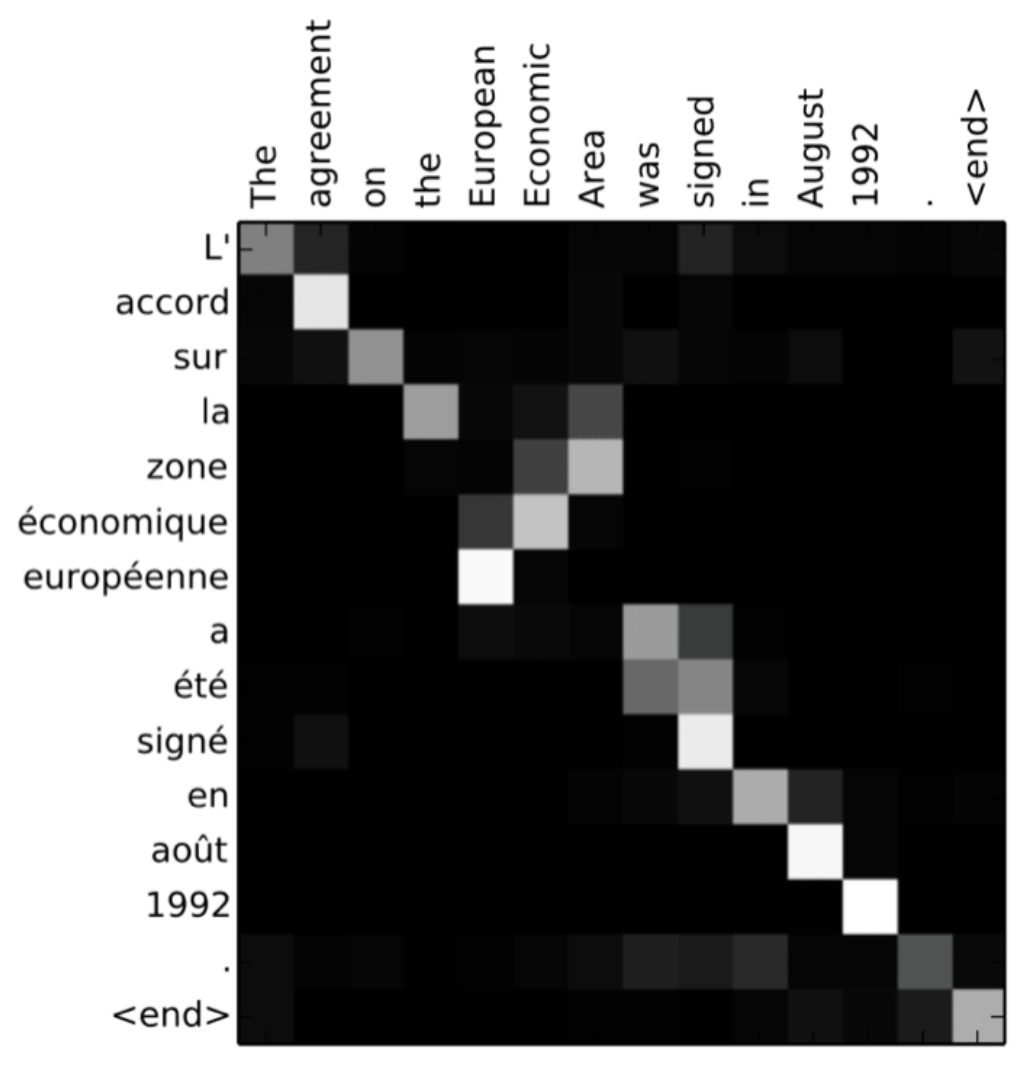
\includegraphics[width=\linewidth]{images/heatmap.png}
    \end{minipage}
    \hfill
    \begin{minipage}{0.45\textwidth}
        \centering
        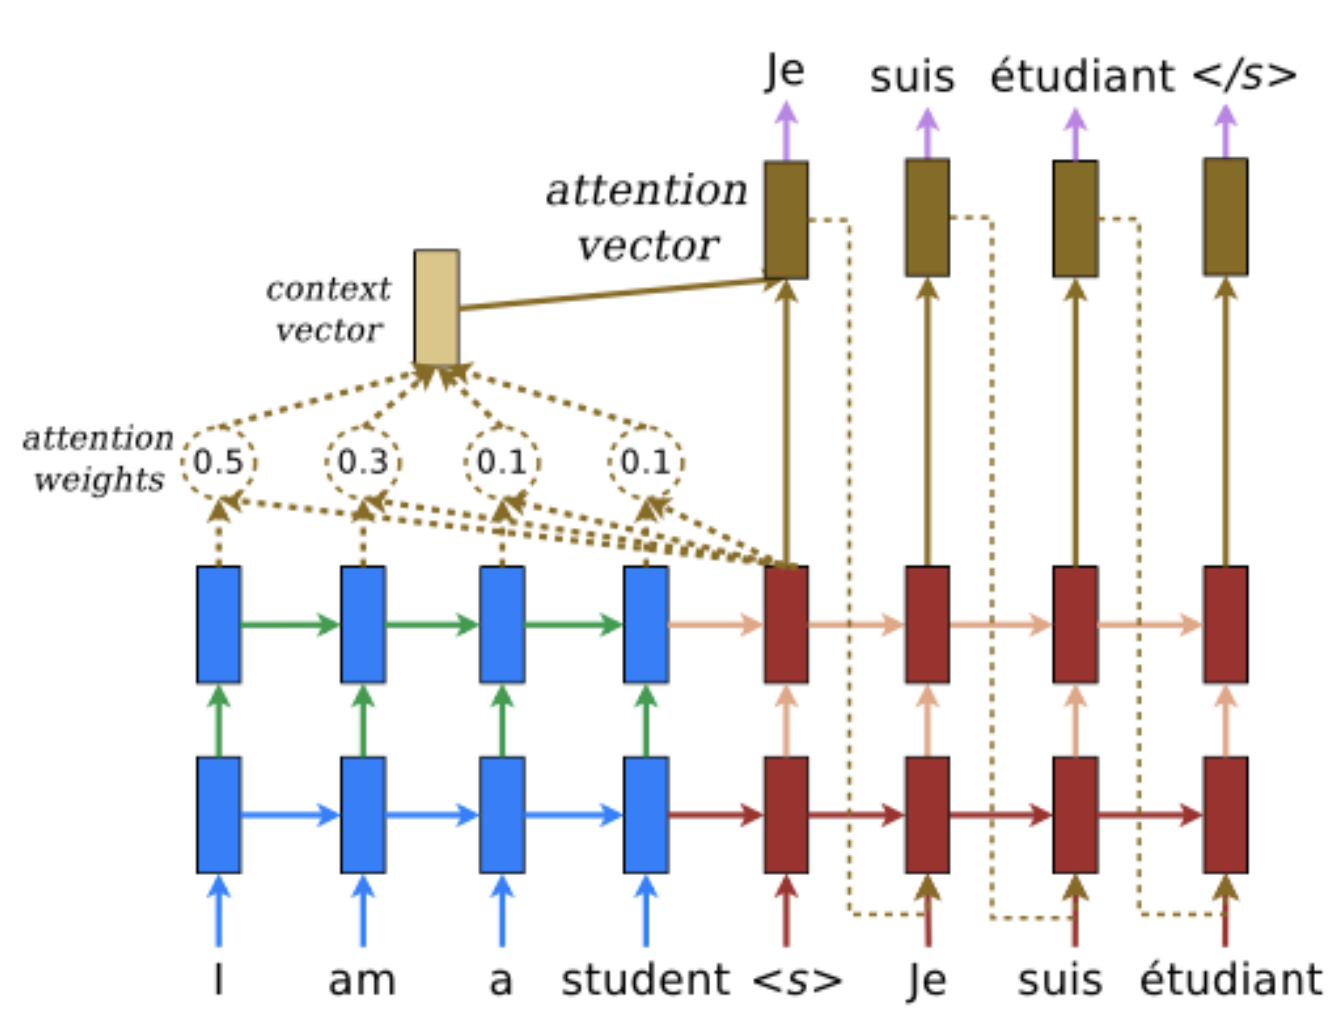
\includegraphics[width=\linewidth]{images/seq2seq-attention-detailed.png}
    \end{minipage}
    \caption{Attention heatmap and output. The heatmap shows which input words are used for each output word. At each step, the decoder computes a context vector by attending to all encoder states. This reveals an alignment between source and target sequences.}
	
    \label{fig:heatmap-and-output}
\end{figure}

\subsection{Self-Attention}

Self-attention layer is the core building block in transformers. Given an input set/sequence of vectors, we now generate an output sequence/set of vectors.

Given input $x_1, \dots, x_T$, we compute query $q_t = W_q x_t$, key $k_t = W_k x_t$, and value $v_t = W_v x_t$ value for each. We then generate each outputs $y_1, \dots, y_T$ using the attention mechanism:

\[ y_t = \text{Attn}(q_t, (k_1, v_1), \dots, (k_T, v_T)) \]

\begin{figure}[htbp]
    \centering
    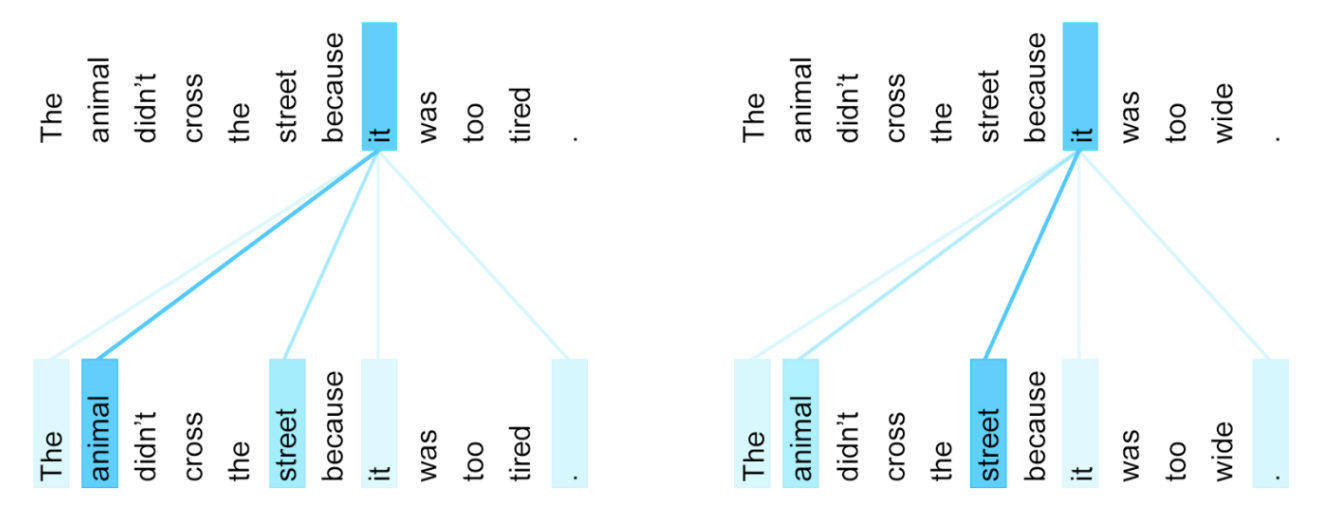
\includegraphics[width=0.6\linewidth]{images/degrees.png}
    \caption{Self attention in transformers. The same word "it" can attend to different words. Each output, pays attention to each input to varying degree we can learn the weights to pay attention to what is relevant for each outpur}
    \label{fig:degreess}
\end{figure}

We can use \textbf{dot product attention} for the entire input:

\begin{figure}[htbp]
    \centering
    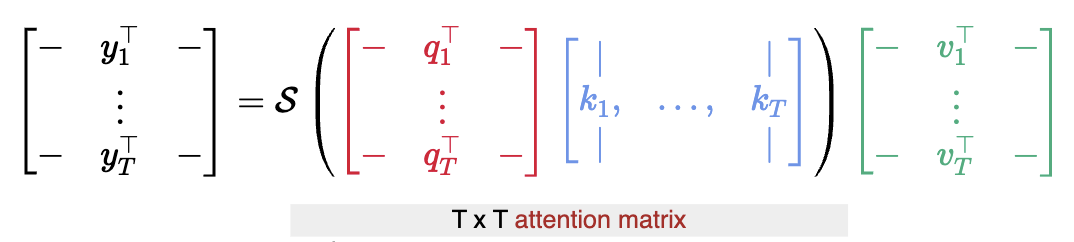
\includegraphics[width=0.7\linewidth]{images/cdot.png}
\end{figure}

Each row sums to one. Each row of the attention matrix gives a linear combination of rows of $V$. We can use an \textbf{attention mask} to prevent some outputs from attenting parts of input. For example a \textbf{causal mask} prevents looking into the future in sequence generation.

\begin{figure}[htbp]
    \centering
    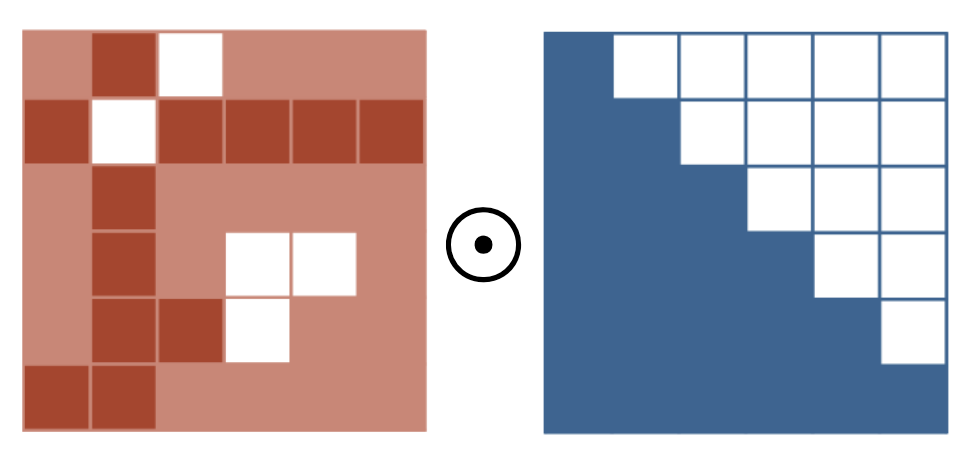
\includegraphics[width=0.4\linewidth]{images/mask.png}
    \caption{Attention mask. We can optionally multiply the attention matrix by a mask matrix so that predictions don't look into the future}
\end{figure}

We often use \textbf{scaled dot-product attention} in practice. The short matrix form of self-attention:

\begin{figure}[H]
    \centering
    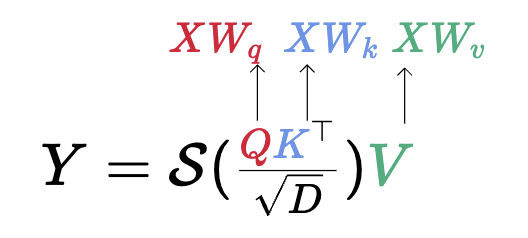
\includegraphics[width=0.3\linewidth]{images/self-attention-matrix-form.png}
\end{figure}

\subsection{Multi-headed Attention}

Multiple attention "heads" can detect different types of relationships/patterns. They use different attention weights:

\begin{figure}[H]
    \centering
    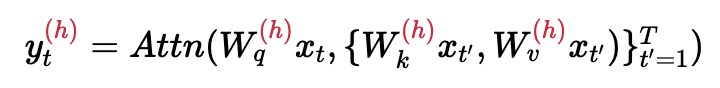
\includegraphics[width=0.55\linewidth]{images/mhattn.png}
\end{figure}


\end{document}
